% Options for packages loaded elsewhere
\PassOptionsToPackage{unicode}{hyperref}
\PassOptionsToPackage{hyphens}{url}
%
\documentclass[
  ignorenonframetext,
]{beamer}
\usepackage{pgfpages}
\setbeamertemplate{caption}[numbered]
\setbeamertemplate{caption label separator}{: }
\setbeamercolor{caption name}{fg=normal text.fg}
\beamertemplatenavigationsymbolsempty
% Prevent slide breaks in the middle of a paragraph
\widowpenalties 1 10000
\raggedbottom
\setbeamertemplate{part page}{
  \centering
  \begin{beamercolorbox}[sep=16pt,center]{part title}
    \usebeamerfont{part title}\insertpart\par
  \end{beamercolorbox}
}
\setbeamertemplate{section page}{
  \centering
  \begin{beamercolorbox}[sep=12pt,center]{part title}
    \usebeamerfont{section title}\insertsection\par
  \end{beamercolorbox}
}
\setbeamertemplate{subsection page}{
  \centering
  \begin{beamercolorbox}[sep=8pt,center]{part title}
    \usebeamerfont{subsection title}\insertsubsection\par
  \end{beamercolorbox}
}
\AtBeginPart{
  \frame{\partpage}
}
\AtBeginSection{
  \ifbibliography
  \else
    \frame{\sectionpage}
  \fi
}
\AtBeginSubsection{
  \frame{\subsectionpage}
}
\usepackage{lmodern}
\usepackage{amssymb,amsmath}
\usepackage{ifxetex,ifluatex}
\ifnum 0\ifxetex 1\fi\ifluatex 1\fi=0 % if pdftex
  \usepackage[T1]{fontenc}
  \usepackage[utf8]{inputenc}
  \usepackage{textcomp} % provide euro and other symbols
\else % if luatex or xetex
  \usepackage{unicode-math}
  \defaultfontfeatures{Scale=MatchLowercase}
  \defaultfontfeatures[\rmfamily]{Ligatures=TeX,Scale=1}
\fi
\usetheme[]{Berlin}
% Use upquote if available, for straight quotes in verbatim environments
\IfFileExists{upquote.sty}{\usepackage{upquote}}{}
\IfFileExists{microtype.sty}{% use microtype if available
  \usepackage[]{microtype}
  \UseMicrotypeSet[protrusion]{basicmath} % disable protrusion for tt fonts
}{}
\makeatletter
\@ifundefined{KOMAClassName}{% if non-KOMA class
  \IfFileExists{parskip.sty}{%
    \usepackage{parskip}
  }{% else
    \setlength{\parindent}{0pt}
    \setlength{\parskip}{6pt plus 2pt minus 1pt}}
}{% if KOMA class
  \KOMAoptions{parskip=half}}
\makeatother
\usepackage{xcolor}
\IfFileExists{xurl.sty}{\usepackage{xurl}}{} % add URL line breaks if available
\IfFileExists{bookmark.sty}{\usepackage{bookmark}}{\usepackage{hyperref}}
\hypersetup{
  pdftitle={Binary Response and Logistic Regression},
  pdfauthor={Marvin Schmitt},
  hidelinks,
  pdfcreator={LaTeX via pandoc}}
\urlstyle{same} % disable monospaced font for URLs
\newif\ifbibliography
\usepackage{color}
\usepackage{fancyvrb}
\newcommand{\VerbBar}{|}
\newcommand{\VERB}{\Verb[commandchars=\\\{\}]}
\DefineVerbatimEnvironment{Highlighting}{Verbatim}{commandchars=\\\{\}}
% Add ',fontsize=\small' for more characters per line
\usepackage{framed}
\definecolor{shadecolor}{RGB}{248,248,248}
\newenvironment{Shaded}{\begin{snugshade}}{\end{snugshade}}
\newcommand{\AlertTok}[1]{\textcolor[rgb]{0.94,0.16,0.16}{#1}}
\newcommand{\AnnotationTok}[1]{\textcolor[rgb]{0.56,0.35,0.01}{\textbf{\textit{#1}}}}
\newcommand{\AttributeTok}[1]{\textcolor[rgb]{0.77,0.63,0.00}{#1}}
\newcommand{\BaseNTok}[1]{\textcolor[rgb]{0.00,0.00,0.81}{#1}}
\newcommand{\BuiltInTok}[1]{#1}
\newcommand{\CharTok}[1]{\textcolor[rgb]{0.31,0.60,0.02}{#1}}
\newcommand{\CommentTok}[1]{\textcolor[rgb]{0.56,0.35,0.01}{\textit{#1}}}
\newcommand{\CommentVarTok}[1]{\textcolor[rgb]{0.56,0.35,0.01}{\textbf{\textit{#1}}}}
\newcommand{\ConstantTok}[1]{\textcolor[rgb]{0.00,0.00,0.00}{#1}}
\newcommand{\ControlFlowTok}[1]{\textcolor[rgb]{0.13,0.29,0.53}{\textbf{#1}}}
\newcommand{\DataTypeTok}[1]{\textcolor[rgb]{0.13,0.29,0.53}{#1}}
\newcommand{\DecValTok}[1]{\textcolor[rgb]{0.00,0.00,0.81}{#1}}
\newcommand{\DocumentationTok}[1]{\textcolor[rgb]{0.56,0.35,0.01}{\textbf{\textit{#1}}}}
\newcommand{\ErrorTok}[1]{\textcolor[rgb]{0.64,0.00,0.00}{\textbf{#1}}}
\newcommand{\ExtensionTok}[1]{#1}
\newcommand{\FloatTok}[1]{\textcolor[rgb]{0.00,0.00,0.81}{#1}}
\newcommand{\FunctionTok}[1]{\textcolor[rgb]{0.00,0.00,0.00}{#1}}
\newcommand{\ImportTok}[1]{#1}
\newcommand{\InformationTok}[1]{\textcolor[rgb]{0.56,0.35,0.01}{\textbf{\textit{#1}}}}
\newcommand{\KeywordTok}[1]{\textcolor[rgb]{0.13,0.29,0.53}{\textbf{#1}}}
\newcommand{\NormalTok}[1]{#1}
\newcommand{\OperatorTok}[1]{\textcolor[rgb]{0.81,0.36,0.00}{\textbf{#1}}}
\newcommand{\OtherTok}[1]{\textcolor[rgb]{0.56,0.35,0.01}{#1}}
\newcommand{\PreprocessorTok}[1]{\textcolor[rgb]{0.56,0.35,0.01}{\textit{#1}}}
\newcommand{\RegionMarkerTok}[1]{#1}
\newcommand{\SpecialCharTok}[1]{\textcolor[rgb]{0.00,0.00,0.00}{#1}}
\newcommand{\SpecialStringTok}[1]{\textcolor[rgb]{0.31,0.60,0.02}{#1}}
\newcommand{\StringTok}[1]{\textcolor[rgb]{0.31,0.60,0.02}{#1}}
\newcommand{\VariableTok}[1]{\textcolor[rgb]{0.00,0.00,0.00}{#1}}
\newcommand{\VerbatimStringTok}[1]{\textcolor[rgb]{0.31,0.60,0.02}{#1}}
\newcommand{\WarningTok}[1]{\textcolor[rgb]{0.56,0.35,0.01}{\textbf{\textit{#1}}}}
\usepackage{graphicx,grffile}
\makeatletter
\def\maxwidth{\ifdim\Gin@nat@width>\linewidth\linewidth\else\Gin@nat@width\fi}
\def\maxheight{\ifdim\Gin@nat@height>\textheight\textheight\else\Gin@nat@height\fi}
\makeatother
% Scale images if necessary, so that they will not overflow the page
% margins by default, and it is still possible to overwrite the defaults
% using explicit options in \includegraphics[width, height, ...]{}
\setkeys{Gin}{width=\maxwidth,height=\maxheight,keepaspectratio}
% Set default figure placement to htbp
\makeatletter
\def\fps@figure{htbp}
\makeatother
\setlength{\emergencystretch}{3em} % prevent overfull lines
\providecommand{\tightlist}{%
  \setlength{\itemsep}{0pt}\setlength{\parskip}{0pt}}
\setcounter{secnumdepth}{-\maxdimen} % remove section numbering
\setbeamertemplate{footline}{}

\title{Binary Response and Logistic Regression}
\author{Marvin Schmitt}
\date{May 11, 2021}

\begin{document}
\frame{\titlepage}

\begin{frame}
  \tableofcontents[hideallsubsections]
\end{frame}
\hypertarget{model}{%
\section{Model}\label{model}}

\begin{frame}{Binary Response Data}
\protect\hypertarget{binary-response-data}{}

\begin{itemize}
\tightlist
\item
  \textbf{General setting:} \(x_i\in\mathbb{R}^n, y_i\in\{0,1\}\)
\item
  \textbf{Examples:}

  \begin{itemize}
  \tightlist
  \item
    Stimulus discrimination tasks

    \begin{itemize}
    \tightlist
    \item
      Shooter paradigm
    \item
      Just noticeable difference in color perception
    \end{itemize}
  \item
    Mortality

    \begin{itemize}
    \tightlist
    \item
      \emph{Is regular physical exercise life extending?}
    \item
      \emph{What are risk factors for severe COVID-19 symptoms?}
    \end{itemize}
  \item
    Performance assessment

    \begin{itemize}
    \tightlist
    \item
      Student assessment tests
    \item
      Exam design: modeling task difficulty
    \end{itemize}
  \end{itemize}
\end{itemize}

\end{frame}

\begin{frame}{Estimation}
\protect\hypertarget{estimation}{}

\textbf{Basic idea:} predict probability for class 1 as
\(P(Y=1)=\dfrac{\exp(\eta)}{1+\exp(\eta)}\) with
\(\eta=\beta_0+\beta_1x_1+\ldots +\beta_kx_k\)

\begin{itemize}
\tightlist
\item
  Underlying linear model
  \(\eta_i = \beta_0+\sum\limits_{j=1}^k\beta_jx_j\) that is plugged
  into the logistic function to obtain \(P(Y=1)\in[0, 1]\) and
  \(P(Y=1)+P(Y\neq1)=1\).
\end{itemize}

\end{frame}

\begin{frame}{Likelihood}
\protect\hypertarget{likelihood}{}

Likelihood
\(\mathcal{L}(\beta|x_1,\ldots,x_n)=\prod_{i=1}^n \mathcal{L}_i(\beta|x_i)\)
\[\begin{aligned}
  \mathit{l}(\beta|x_1,\ldots,x_n)& =\sum_{i=1}^n l_i(\beta|x_i)\\
  &=\sum (1-y_i)\log(1-p(x_i;\beta)) + y_i\log p(x_i;\beta)\\
  &=\sum y_i\log\dfrac{p(x_i;\beta)}{1-p(x_i;\beta)}+\log(1-p(x_i;\beta))\\
  &=\sum y_ix_i\beta - \log(1+\exp(x_i\beta))\\
  &=\sum_{i=1}^ny_i\eta_i-\log(1+\exp(\eta))
\end{aligned}\]

\begin{itemize}
\tightlist
\item
  Maximize log-likelihood
  \(l=\sum_{i=1}^ny_i\eta_i-\log(1+\exp(\eta))=:\mathtt{LL}\)
\end{itemize}

\end{frame}

\begin{frame}[fragile]{Inference}
\protect\hypertarget{inference}{}

\begin{itemize}
\tightlist
\item
  \textbf{Data format}

  \begin{itemize}
  \tightlist
  \item
    The criterion must be coded as \texttt{0/1} or as \texttt{factor}.
  \item
    Predictors must be metric or dummy-coded
  \end{itemize}
\item
  \textbf{Interpretation}

  \begin{itemize}
  \tightlist
  \item
    Odds ratio for predictor \(x_j\) is equal to \(\exp(\beta_j)\)
  \item
    Odds ratio \(OR_j\) quantifies how the odds
    \(\frac{P(Y=1)}{P(Y=0)}\) change when \(x_j\) increases by 1 unit.
  \end{itemize}
\end{itemize}

\end{frame}

\hypertarget{implementation-in-r}{%
\section{\texorpdfstring{Implementation in
\texttt{R}}{Implementation in R}}\label{implementation-in-r}}

\begin{frame}[fragile]{Syntax}
\protect\hypertarget{syntax}{}

\textbf{General syntax}

\begin{itemize}
\tightlist
\item
  Command \texttt{glm()} (generalized linear model)
\item
  Formula syntax:

  \begin{itemize}
  \tightlist
  \item
    \texttt{y\textasciitilde{}x1+x2+x3} (no interactions)
  \item
    \texttt{y\textasciitilde{}x1*x2} (interactions)
  \item
    \texttt{y\textasciitilde{}x1+x2+x3+x1:x2} (selected interactions)
  \end{itemize}
\item
  Must provide a \texttt{link} function to \texttt{glm()} through the
  \texttt{family} parameter (cf.~section
  \protect\hyperlink{other-link-functions}{Other link functions})

  \begin{itemize}
  \tightlist
  \item
    For logistic regression, we use
    \texttt{family=binomial(\textquotesingle{}logit\textquotesingle{})}.
  \end{itemize}
\end{itemize}

\textbf{Examples} \tiny

\begin{Shaded}
\begin{Highlighting}[]
\NormalTok{m1 =}\StringTok{ }\KeywordTok{glm}\NormalTok{(correct_response }\OperatorTok{~}\StringTok{ }\NormalTok{iq }\OperatorTok{+}\StringTok{ }\NormalTok{math_skill, }\DataTypeTok{data=}\NormalTok{df, }\DataTypeTok{family=}\KeywordTok{binomial}\NormalTok{(}\StringTok{'logit'}\NormalTok{))}
\NormalTok{m2 =}\StringTok{ }\KeywordTok{glm}\NormalTok{(fatal_accident }\OperatorTok{~}\StringTok{ }\NormalTok{bmi }\OperatorTok{+}\StringTok{ }\NormalTok{risk_seeking }\OperatorTok{+}\StringTok{ }\NormalTok{gender, }\DataTypeTok{family=}\KeywordTok{binomial}\NormalTok{(}\StringTok{'logit'}\NormalTok{))}
\NormalTok{m3 =}\StringTok{ }\KeywordTok{glm}\NormalTok{(vaccination_skeptic }\OperatorTok{~}\StringTok{ }\NormalTok{iq }\OperatorTok{*}\StringTok{ }\NormalTok{income, }\DataTypeTok{family=}\KeywordTok{binomial}\NormalTok{(}\StringTok{'logit'}\NormalTok{))}
\end{Highlighting}
\end{Shaded}

\normalsize

\end{frame}

\begin{frame}[fragile]{Toy Example}
\protect\hypertarget{toy-example}{}

The dataset \texttt{df}\footnote<.->{\textless www.github.com/marvinschmitt/talk-binary-response\textgreater{}}
contains the yearly sick leave hours, number of tweets on Twitter, IQ,
and hair length of \(N=100\) employees along with their gender (binary:
male/female) and whether they have ever suffered from depression
(binary: yes/no):

\tiny

\begin{Shaded}
\begin{Highlighting}[]
\NormalTok{df }\OperatorTok\StringTok{ }\KeywordTok{slice}\NormalTok{(}\KeywordTok{sample}\NormalTok{(}\KeywordTok{nrow}\NormalTok{(df))) }\OperatorTok\StringTok{ }\KeywordTok{head}\NormalTok{(}\DecValTok{5}\NormalTok{)}
\end{Highlighting}
\end{Shaded}

\begin{verbatim}
##   ID depr gender avg_sickhours n_tweets iq hairlength
## 1 75   no   male          13.0        3 90       19.5
## 2 91   no   male          12.7        3 84        4.8
## 3 23  yes female          11.5       12 90       46.3
## 4 33   no female           5.4        3 97       40.4
## 5 86   no   male           8.6        1 83        4.4
\end{verbatim}

\begin{Shaded}
\begin{Highlighting}[]
\KeywordTok{table}\NormalTok{(df}\OperatorTok{$}\NormalTok{gender)}
\end{Highlighting}
\end{Shaded}

\begin{verbatim}
## 
## female   male 
##     50     50
\end{verbatim}

\normalsize

\end{frame}

\begin{frame}[fragile]

We define \texttt{gender} as criterion and \texttt{avg\_sickhours} as
predictor. The \texttt{logit} link function leads to a logistic
regression. The output's coefficients correspond to
\(\beta_0,\ldots,\beta_k\).

\tiny

\begin{Shaded}
\begin{Highlighting}[]
\NormalTok{m =}\StringTok{ }\KeywordTok{glm}\NormalTok{(gender }\OperatorTok{~}\StringTok{ }\NormalTok{avg_sickhours, }\DataTypeTok{data =}\NormalTok{ df, }\DataTypeTok{family =} \KeywordTok{binomial}\NormalTok{(}\StringTok{'logit'}\NormalTok{))}
\NormalTok{m}\OperatorTok{$}\NormalTok{coefficients}
\end{Highlighting}
\end{Shaded}

\begin{verbatim}
##   (Intercept) avg_sickhours 
##    -4.2693393     0.4440937
\end{verbatim}

\normalsize
\tiny\normalsize

\begin{itemize}
\tightlist
\item
  We can calculate \(\eta\) from the underlying linear model:
  \(\eta= -4.27 + 0.44 x_1\)
\item
  Thus, the criterion estimate is:
  \(\hat{P}(Y=\text{male})=\dfrac{\exp(\overbrace{-4.27 + 0.44 x_1)}^{\eta}}{1+\exp(\underbrace{-4.27 + 0.44 x_1)}_{\eta}}\)
\item
  The odds for \texttt{gender=m} are increased by the factor
  \(\exp(0.44)=1.55\) per additional sick leave hour.
\end{itemize}

\end{frame}

\begin{frame}

\tiny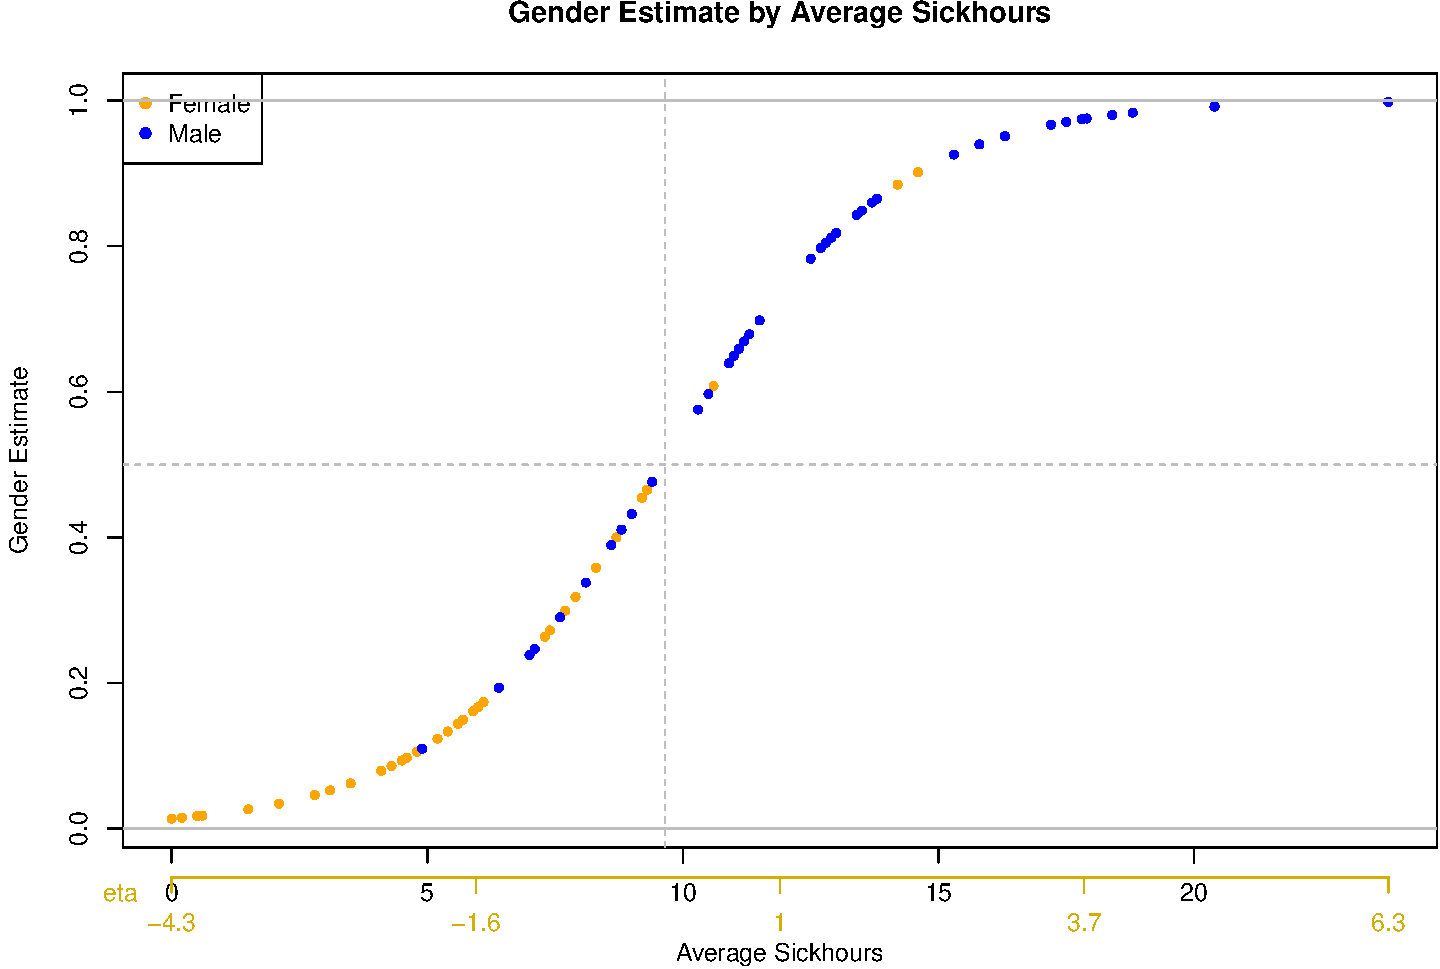
\includegraphics{Schmitt_Marvin_binary_response_files/figure-beamer/TOY_LOG_PLOT-1.pdf}
\normalsize

\end{frame}

\begin{frame}[fragile]

\textbf{Predictors:} Avg. sick hours (\(x_1\)), Number of tweets
(\(x_2\))

\tiny

\begin{Shaded}
\begin{Highlighting}[]
\NormalTok{m =}\StringTok{ }\KeywordTok{glm}\NormalTok{(gender }\OperatorTok{~}\StringTok{ }\NormalTok{avg_sickhours }\OperatorTok{+}\StringTok{ }\NormalTok{n_tweets, }\DataTypeTok{data =}\NormalTok{ df, }\DataTypeTok{family =} \KeywordTok{binomial}\NormalTok{(}\StringTok{'logit'}\NormalTok{))}
\NormalTok{m}\OperatorTok{$}\NormalTok{coefficients}
\end{Highlighting}
\end{Shaded}

\begin{verbatim}
##   (Intercept) avg_sickhours      n_tweets 
##    -10.109104      1.621815     -1.197958
\end{verbatim}

\normalsize
\tiny\normalsize

\begin{itemize}
\tightlist
\item
  \(\eta= -10.11 + 1.62 x_1 + -1.2 x_2\)
\end{itemize}

\tiny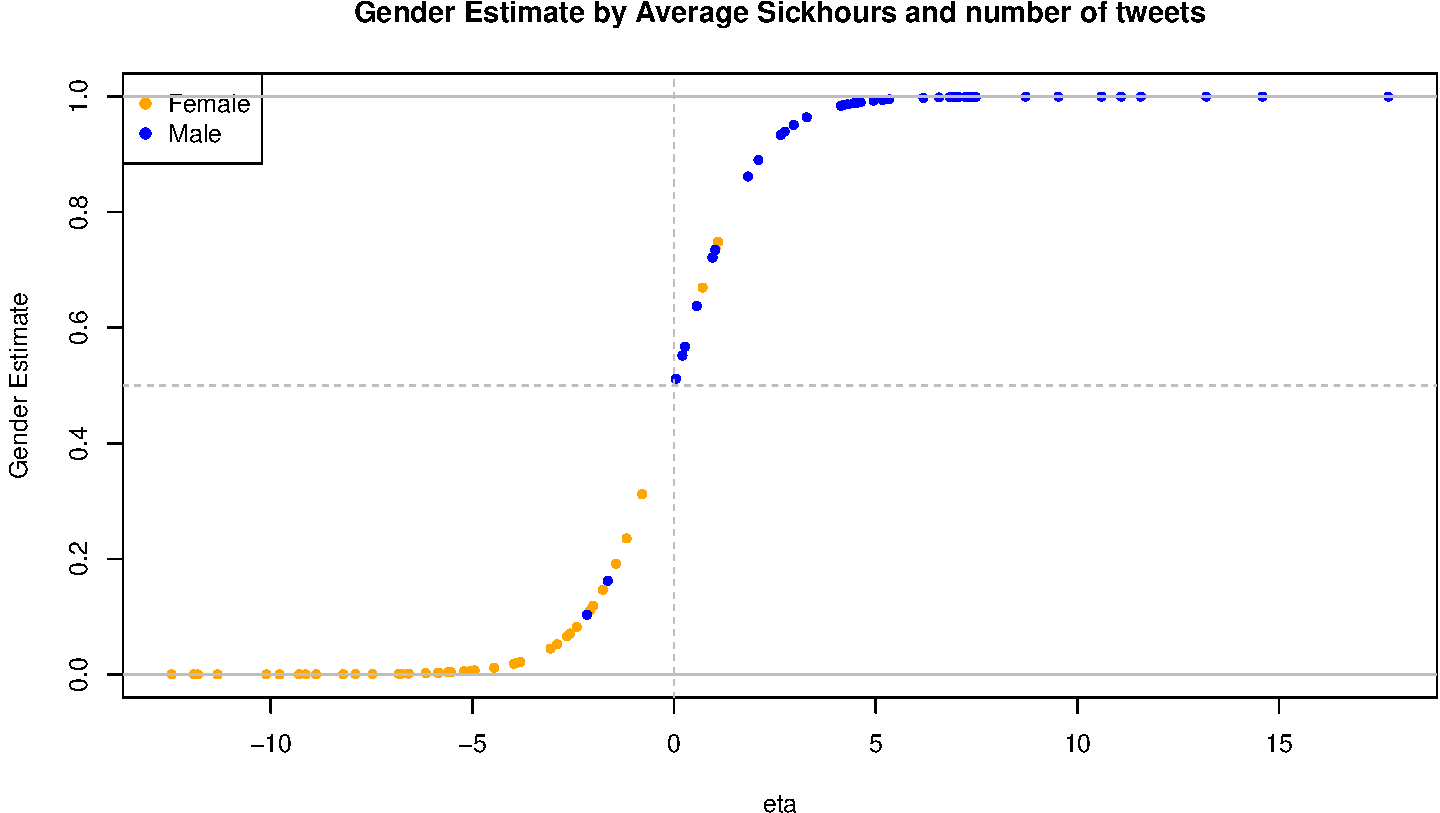
\includegraphics{Schmitt_Marvin_binary_response_files/figure-beamer/unnamed-chunk-8-1.pdf}
\normalsize

\end{frame}

\begin{frame}[fragile]

\textbf{Predictors:} Avg. sick hours (\(x_1\)), Number of tweets
(\(x_2\)), IQ (\(x_3\))

\tiny

\begin{Shaded}
\begin{Highlighting}[]
\NormalTok{m =}\StringTok{ }\KeywordTok{glm}\NormalTok{(gender }\OperatorTok{~}\StringTok{ }\NormalTok{avg_sickhours }\OperatorTok{+}\StringTok{ }\NormalTok{n_tweets }\OperatorTok{+}\StringTok{ }\NormalTok{iq, }\DataTypeTok{data =}\NormalTok{ df, }\DataTypeTok{family =} \KeywordTok{binomial}\NormalTok{(}\StringTok{'logit'}\NormalTok{))}
\end{Highlighting}
\end{Shaded}

\begin{verbatim}
## Warning: glm.fit: algorithm did not converge
\end{verbatim}

\begin{verbatim}
## Warning: glm.fit: fitted probabilities numerically 0 or 1 occurred
\end{verbatim}

\begin{Shaded}
\begin{Highlighting}[]
\NormalTok{m}\OperatorTok{$}\NormalTok{coefficients}
\end{Highlighting}
\end{Shaded}

\begin{verbatim}
##   (Intercept) avg_sickhours      n_tweets            iq 
##    1998.03388     150.38876     -79.29431     -33.13080
\end{verbatim}

\normalsize
\tiny\normalsize

\begin{itemize}
\item
  \(\eta= 1998.03 + 150.39 x_1 + -79.29 x_2 + -33.13 x_3\)
\item
  Note the output
  \texttt{Warning:\ glm.fit:\ algorithm\ did\ not\ converge}

  \begin{itemize}
  \tightlist
  \item
    Issue: Data is linearly separable (cf.~section
    \protect\hyperlink{issue-linear-separability}{Issue: Linear
    Separability})
  \item
    See the plot (next slide)
  \end{itemize}
\end{itemize}

\end{frame}

\begin{frame}

\tiny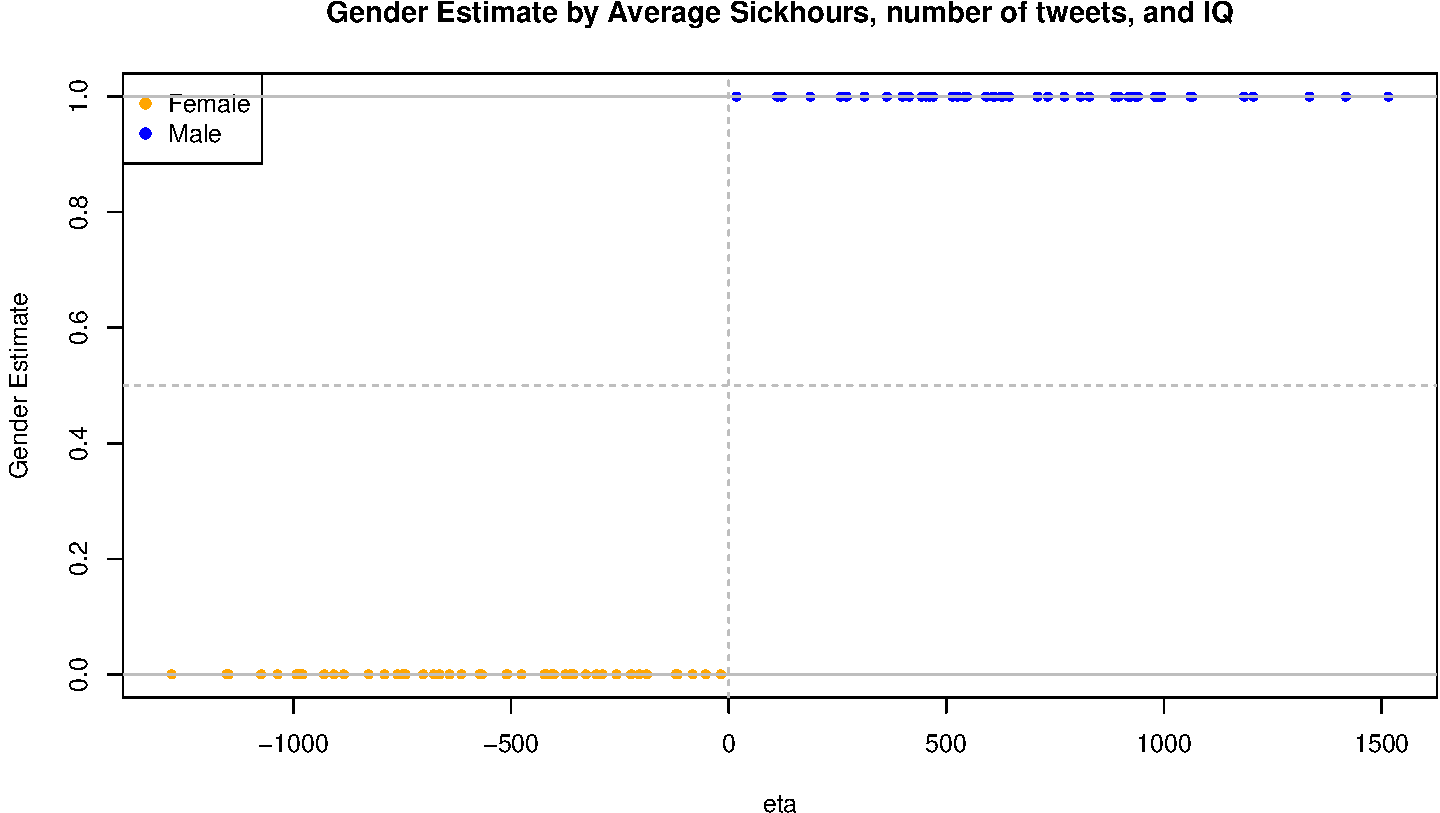
\includegraphics{Schmitt_Marvin_binary_response_files/figure-beamer/unnamed-chunk-11-1.pdf}
\normalsize

\end{frame}

\begin{frame}[fragile]

\textbf{Predictors:} Avg. sick hours (\(x_1\)), Hairlength (\(x_2\))

\tiny

\begin{Shaded}
\begin{Highlighting}[]
\NormalTok{m =}\StringTok{ }\KeywordTok{glm}\NormalTok{(gender }\OperatorTok{~}\StringTok{ }\NormalTok{avg_sickhours }\OperatorTok{+}\StringTok{ }\NormalTok{hairlength, }\DataTypeTok{data =}\NormalTok{ df, }\DataTypeTok{family =} \KeywordTok{binomial}\NormalTok{(}\StringTok{'logit'}\NormalTok{))}
\end{Highlighting}
\end{Shaded}

\begin{verbatim}
## Warning: glm.fit: algorithm did not converge
\end{verbatim}

\begin{verbatim}
## Warning: glm.fit: fitted probabilities numerically 0 or 1 occurred
\end{verbatim}

\normalsize

\tiny

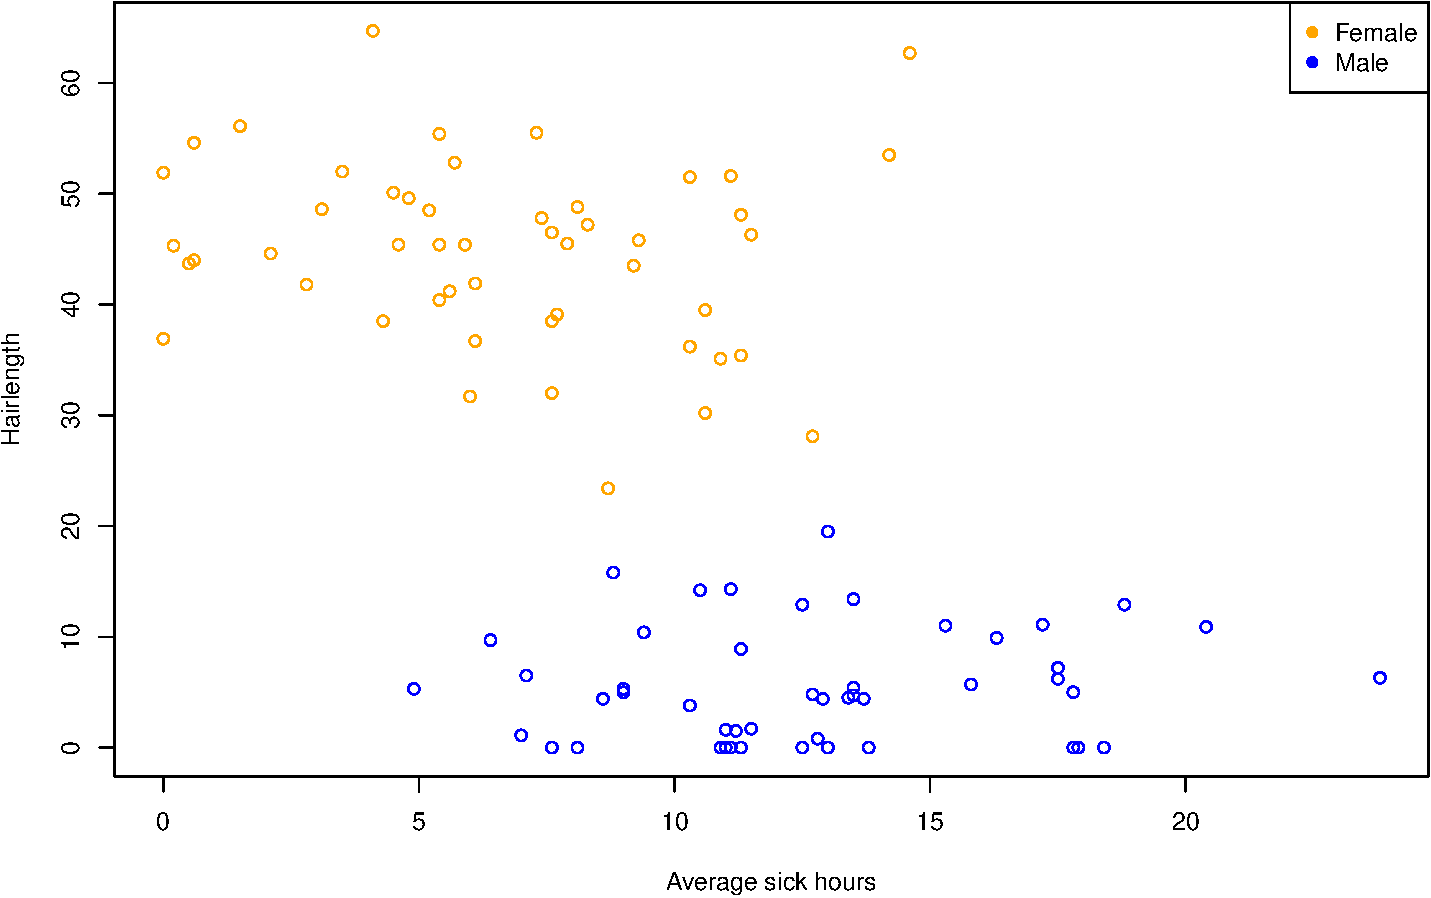
\includegraphics[width=7\linewidth,height=0.7\textheight]{Schmitt_Marvin_binary_response_files/figure-beamer/unnamed-chunk-13-1}
\normalsize

\end{frame}

\hypertarget{model-evaluation}{%
\section{Model Evaluation}\label{model-evaluation}}

\begin{frame}{Logarithmic Scoring}
\protect\hypertarget{logarithmic-scoring}{}

\begin{itemize}
\tightlist
\item
  Basic evaluation of predicted probabilities:

  \begin{itemize}
  \tightlist
  \item
    For \(Y_{true}=1\), the predicted probability \(\hat{P}(Y=1)\)
    should be close to 1.
  \item
    For \(Y_{true}=0\), the predicted probability \(\hat{P}(Y=1)\)
    should be close to 0.
  \end{itemize}
\item
  Compute
  \(\mathtt{logScore}=Y_i\ln(\hat{Y}_i)+(1-Y_i)\ln(1-\hat{Y}_i)\)

  \begin{itemize}
  \tightlist
  \item
    \(=\ln(\hat{Y_i}) \quad\text{if}\quad Y_i=1\)
  \item
    \(=\ln(1-\hat{Y_i}) \quad\text{if}\quad Y_i=0\)
  \end{itemize}
\end{itemize}

\end{frame}

\begin{frame}[fragile]{Model Selection}
\protect\hypertarget{model-selection}{}

\begin{itemize}
\tightlist
\item
  Model selection aims at selecting a model \(M_i\) from a set of
  candidate models \(M_1,\ldots,M_m\).
\item
  The choice depends on the selection criterion and the
\item
  For a model \emph{M} with \emph{k} parameters, the
  \textbf{Akaike-Information-Criterion} is defined as
\end{itemize}

\[AIC_M=-2\log L_M+2k\] - \texttt{R} provides the \texttt{step()}
function for stepwise selection from a set of models\footnote<.->{stepwise
  selection is not an ideal selection technique. Contemporary
  alternative: regularized methods}. - The \texttt{step()} function uses
the \(AIC\) as selection criterion for logistic regression models.

\end{frame}

\begin{frame}[fragile]

\tiny

\begin{Shaded}
\begin{Highlighting}[]
\NormalTok{m0 =}\StringTok{ }\KeywordTok{glm}\NormalTok{(chd}\OperatorTok{~}\DecValTok{1}\NormalTok{, }\DataTypeTok{data=}\NormalTok{chd_data, }\DataTypeTok{family=}\KeywordTok{binomial}\NormalTok{(}\StringTok{'logit'}\NormalTok{))}
\NormalTok{m1 =}\StringTok{ }\KeywordTok{step}\NormalTok{(m0, }\DataTypeTok{direction=}\StringTok{'both'}\NormalTok{, }\DataTypeTok{trace=}\DecValTok{0}\NormalTok{,}
          \DataTypeTok{scope=}\StringTok{'~cigs+chol+weight+age'}\NormalTok{)}
\KeywordTok{summary}\NormalTok{(m1)}
\end{Highlighting}
\end{Shaded}

\begin{verbatim}
## 
## Call:
## glm(formula = chd ~ chol + age + cigs, family = binomial("logit"), 
##     data = chd_data)
## 
## Deviance Residuals: 
##     Min       1Q   Median       3Q      Max  
## -1.1307  -0.4596  -0.3550  -0.2587   2.6391  
## 
## Coefficients:
##              Estimate Std. Error z value Pr(>|z|)    
## (Intercept) -8.655131   1.660169  -5.213 1.85e-07 ***
## chol         0.014092   0.003422   4.118 3.82e-05 ***
## age          0.056783   0.029257   1.941   0.0523 .  
## cigs         0.017611   0.010368   1.699   0.0894 .  
## ---
## Signif. codes:  0 '***' 0.001 '**' 0.01 '*' 0.05 '.' 0.1 ' ' 1
## 
## (Dispersion parameter for binomial family taken to be 1)
## 
##     Null deviance: 302.35  on 498  degrees of freedom
## Residual deviance: 276.65  on 495  degrees of freedom
## AIC: 284.65
## 
## Number of Fisher Scoring iterations: 5
\end{verbatim}

\normalsize

\end{frame}

\begin{frame}[fragile]{Likelihood Ratio Test}
\protect\hypertarget{likelihood-ratio-test}{}

\begin{itemize}
\tightlist
\item
  We can test competing nested models with the \textbf{Likelihood Ratio
  (LR) Test}
\item
  Small model \(M_1\) with \(k_1\) parameters, Large model \(M_2\) with
  \(k_2\) parameters
\item
  The difference of log-likelihoods is \(\chi^2\) distributed:

  \begin{itemize}
  \tightlist
  \item
    Test statistic
    \(G^2=-2LL_{M_1} - (-2LL_{M_2}) \sim \chi^2(df=k_2-k_1)\)
  \item
    If \(p<.05\), the larger model improves model fit.
  \end{itemize}
\item
  Implementation in \texttt{R} for example with
  \texttt{anova({[}models{]},\ test=\textquotesingle{}Chisq\textquotesingle{})}
\end{itemize}

\end{frame}

\begin{frame}[fragile]

\tiny

\begin{Shaded}
\begin{Highlighting}[]
\KeywordTok{anova}\NormalTok{(m0, m1, m2, m3, m4, }\DataTypeTok{test=}\StringTok{"Chisq"}\NormalTok{)}
\end{Highlighting}
\end{Shaded}

\begin{verbatim}
## Analysis of Deviance Table
## 
## Model 1: chd ~ 1
## Model 2: chd ~ age
## Model 3: chd ~ age + cigs
## Model 4: chd ~ age + cigs + chol
## Model 5: chd ~ age + cigs + chol + height
##   Resid. Df Resid. Dev Df Deviance  Pr(>Chi)    
## 1       498     302.35                          
## 2       497     296.76  1   5.5866   0.01810 *  
## 3       496     293.78  1   2.9815   0.08422 .  
## 4       495     276.65  1  17.1342 3.483e-05 ***
## 5       494     275.52  1   1.1310   0.28755    
## ---
## Signif. codes:  0 '***' 0.001 '**' 0.01 '*' 0.05 '.' 0.1 ' ' 1
\end{verbatim}

\normalsize

\end{frame}

\begin{frame}[fragile]{Hosmer and Lemeshow Goodness-of-fit test}
\protect\hypertarget{hosmer-and-lemeshow-goodness-of-fit-test}{}

\begin{itemize}
\tightlist
\item
  Approach of the HL test:

  \begin{itemize}
  \tightlist
  \item
    Partition the model population space into bins (\emph{risk
    decentiles})
  \item
    Compare observed relative bin counts with predicted relative bin
    counts
  \item
    Test statistic follows a \(\chi^2\) distribution
  \end{itemize}
\item
  Interpretation

  \begin{itemize}
  \tightlist
  \item
    \(p<.05\) indicates a systematic deviance between observed and
    predicted bin counts.
  \end{itemize}
\item
  Reasons for a bad fit

  \begin{itemize}
  \tightlist
  \item
    Nonlinear influence of predictors on \(\eta\)

    \begin{itemize}
    \tightlist
    \item
      Solution: Polynomial logistic regression
    \item
      e.g.~\(\eta=\beta_0+\beta_{11}x_1+\beta_{12}x_1^2+\ldots+\beta_{1p}x_1^p+\beta_{21}x_2+\ldots+\beta_{kp}x_k^p\)
    \end{itemize}
  \item
    Interaction between predictors

    \begin{itemize}
    \tightlist
    \item
      Solution: Allow and analyze interactions
      (\texttt{y\textasciitilde{}x1*x2}).
    \end{itemize}
  \end{itemize}
\end{itemize}

\end{frame}

\begin{frame}[fragile]

\tiny

\begin{Shaded}
\begin{Highlighting}[]
\NormalTok{df}\OperatorTok{$}\NormalTok{gender01 =}\StringTok{ }\KeywordTok{as.numeric}\NormalTok{(df}\OperatorTok{$}\NormalTok{gender)}\OperatorTok{-}\DecValTok{1}  \CommentTok{# recode to 0/1 for HL-test}
\NormalTok{m =}\StringTok{ }\KeywordTok{glm}\NormalTok{(gender01 }\OperatorTok{~}\StringTok{ }\NormalTok{avg_sickhours, }\DataTypeTok{data=}\NormalTok{df, }\DataTypeTok{family=}\KeywordTok{binomial}\NormalTok{(}\StringTok{'logit'}\NormalTok{))}
\NormalTok{y_hat =}\StringTok{ }\KeywordTok{predict}\NormalTok{(m, }\DataTypeTok{type=}\StringTok{"response"}\NormalTok{)}
\KeywordTok{hoslem.test}\NormalTok{(df}\OperatorTok{$}\NormalTok{gender01, y_hat)  }\CommentTok{# default: g=10 bins}
\end{Highlighting}
\end{Shaded}

\begin{verbatim}
## 
##  Hosmer and Lemeshow goodness of fit (GOF) test
## 
## data:  df$gender01, y_hat
## X-squared = 3.6825, df = 8, p-value = 0.8846
\end{verbatim}

\begin{Shaded}
\begin{Highlighting}[]
\KeywordTok{hoslem.test}\NormalTok{(df}\OperatorTok{$}\NormalTok{gender01, y_hat, }\DataTypeTok{g=}\DecValTok{5}\NormalTok{)  }\CommentTok{# g=5 bins}
\end{Highlighting}
\end{Shaded}

\begin{verbatim}
## 
##  Hosmer and Lemeshow goodness of fit (GOF) test
## 
## data:  df$gender01, y_hat
## X-squared = 0.57315, df = 3, p-value = 0.9026
\end{verbatim}

\normalsize

\end{frame}

\begin{frame}[fragile]{Effect size}
\protect\hypertarget{effect-size}{}

\textbf{McFadden's \(\rho^2\)}

\begin{itemize}
\tightlist
\item
  \textbf{Problem:} We cannot calculate the explained variance \(R^2\)
\item
  \textbf{Approach:} Calculate McFadden's \(\rho^2\) with the
  log-likelihood of the full model \texttt{m1} and the log-likelihood of
  the null model \texttt{m0} without predictors.
\item
  \textbf{Optional:} Include a correction for the number of predictors
  \(k\).
\item
  \textbf{Formula:}
  \(\rho^2=1-\dfrac{\ln(L_1)\overbrace{-k}^{\text{correction}}}{\ln(L_0)}\)
\end{itemize}

\tiny

\begin{Shaded}
\begin{Highlighting}[]
\NormalTok{m0 =}\StringTok{ }\KeywordTok{glm}\NormalTok{(gender }\OperatorTok{~}\StringTok{ }\DecValTok{1}\NormalTok{,             }\DataTypeTok{data=}\NormalTok{df, }\DataTypeTok{family=}\KeywordTok{binomial}\NormalTok{(}\StringTok{'logit'}\NormalTok{))}
\NormalTok{m1 =}\StringTok{ }\KeywordTok{glm}\NormalTok{(gender }\OperatorTok{~}\StringTok{ }\NormalTok{avg_sickhours, }\DataTypeTok{data=}\NormalTok{df, }\DataTypeTok{family=}\KeywordTok{binomial}\NormalTok{(}\StringTok{'logit'}\NormalTok{))}
\NormalTok{K =}\StringTok{ }\KeywordTok{length}\NormalTok{(m1}\OperatorTok{$}\NormalTok{coefficients) }\OperatorTok{-}\StringTok{ }\DecValTok{1} \CommentTok{# number of predictors}
\KeywordTok{as.numeric}\NormalTok{(}\DecValTok{1} \OperatorTok{-}\StringTok{  }\KeywordTok{logLik}\NormalTok{(m1)   }\OperatorTok{/}\KeywordTok{logLik}\NormalTok{(m0)) }\OperatorTok\StringTok{ }\KeywordTok{round}\NormalTok{(}\DecValTok{3}\NormalTok{)}
\end{Highlighting}
\end{Shaded}

\begin{verbatim}
## [1] 0.36
\end{verbatim}

\begin{Shaded}
\begin{Highlighting}[]
\KeywordTok{as.numeric}\NormalTok{(}\DecValTok{1} \OperatorTok{-}\StringTok{ }\NormalTok{(}\KeywordTok{logLik}\NormalTok{(m1)}\OperatorTok{-}\NormalTok{K)}\OperatorTok{/}\KeywordTok{logLik}\NormalTok{(m0)) }\OperatorTok\StringTok{ }\KeywordTok{round}\NormalTok{(}\DecValTok{3}\NormalTok{)}
\end{Highlighting}
\end{Shaded}

\begin{verbatim}
## [1] 0.346
\end{verbatim}

\normalsize

\end{frame}

\begin{frame}[fragile]

\textbf{Nagelkerke's \(R^2\)}

\begin{itemize}
\tightlist
\item
  Another approach to compute an analogon to \(R^2\) is Nagelkerke's
  (pseudo-) \(R^2\):
\end{itemize}

\tiny

\begin{Shaded}
\begin{Highlighting}[]
\NormalTok{m =}\StringTok{ }\KeywordTok{glm}\NormalTok{(gender }\OperatorTok{~}\StringTok{ }\NormalTok{avg_sickhours, }\DataTypeTok{data=}\NormalTok{df, }\DataTypeTok{family=}\KeywordTok{binomial}\NormalTok{(}\StringTok{'logit'}\NormalTok{))}
\NormalTok{N =}\StringTok{ }\KeywordTok{nrow}\NormalTok{(df)}
\NormalTok{(}\DecValTok{1}\OperatorTok{-}\KeywordTok{exp}\NormalTok{((m}\OperatorTok{$}\NormalTok{dev}\OperatorTok{-}\NormalTok{m}\OperatorTok{$}\NormalTok{null)}\OperatorTok{/}\NormalTok{N))}\OperatorTok{/}\NormalTok{(}\DecValTok{1}\OperatorTok{-}\KeywordTok{exp}\NormalTok{(}\OperatorTok{-}\NormalTok{m}\OperatorTok{$}\NormalTok{null}\OperatorTok{/}\NormalTok{N))}
\end{Highlighting}
\end{Shaded}

\begin{verbatim}
## [1] 0.5238511
\end{verbatim}

\normalsize

\end{frame}

\begin{frame}{Issue: Linear Separability}
\protect\hypertarget{issue-linear-separability}{}

\begin{itemize}
\tightlist
\item
  Linear separability of the data causes convergence issues.
\end{itemize}

\tiny

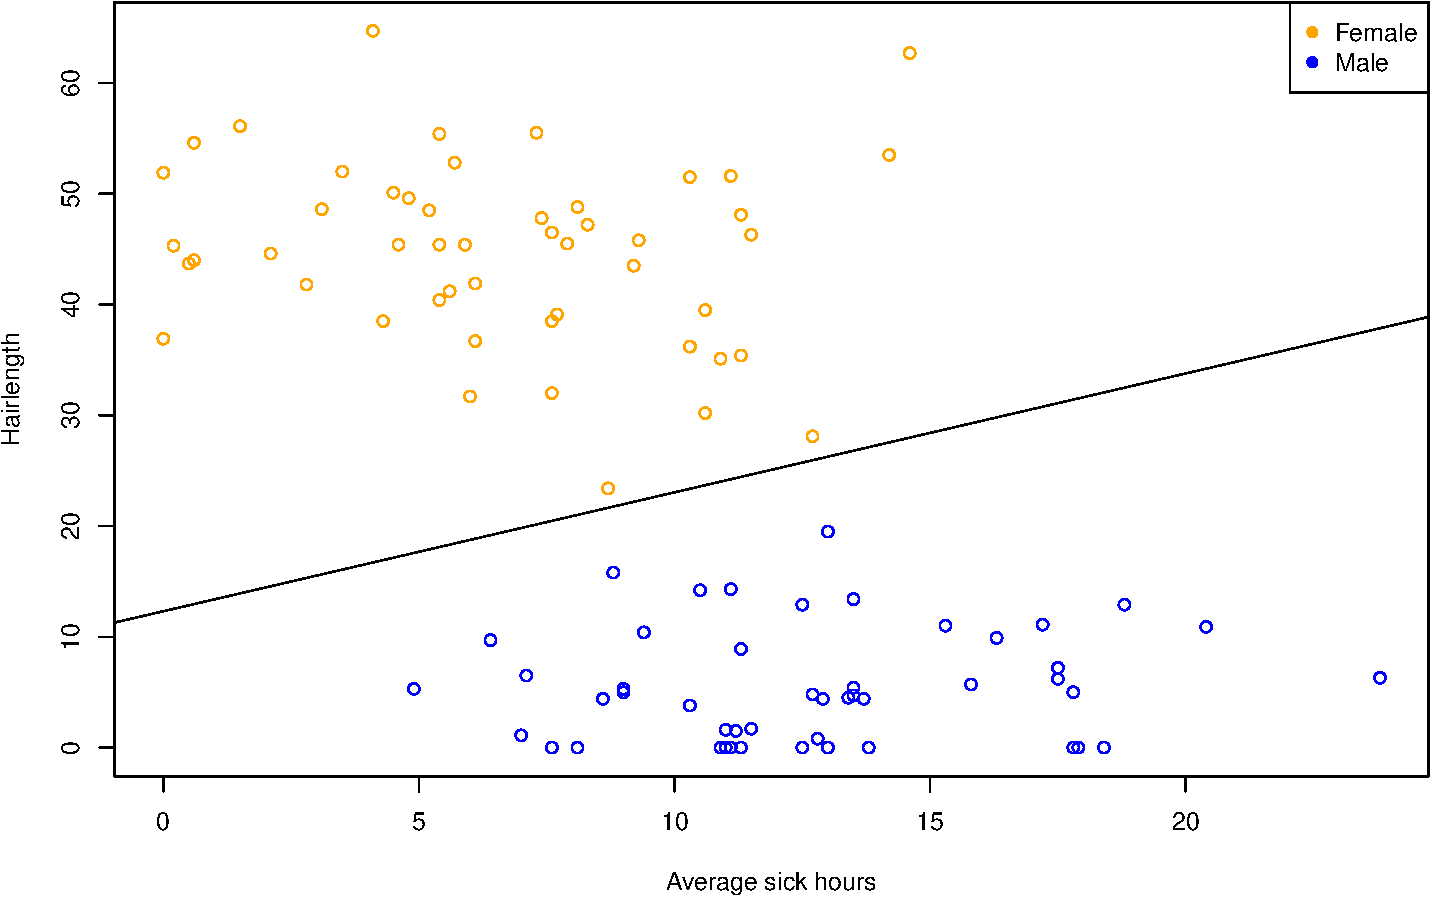
\includegraphics[width=0.5\linewidth,height=0.5\textheight]{Schmitt_Marvin_binary_response_files/figure-beamer/unnamed-chunk-22-1}
\normalsize

\begin{itemize}
\tightlist
\item
  Unstable estimates of the parameters and their standard errors.
\item
  Alternative: \emph{Exact logistic regression}
\end{itemize}

\end{frame}

\hypertarget{outlook}{%
\section{Outlook}\label{outlook}}

\begin{frame}[fragile]{Predictions}
\protect\hypertarget{predictions}{}

\begin{itemize}
\tightlist
\item
  Given a new input \(\dot{x}\), the prediction on the linear predictor
  is \(\hat{\eta}=\dot{x}\hat{\beta}\).
\item
  This prediction \(\eta\) can be equipped with a confidence interval.
\item
  To obtain a probability confidence interval, \(\hat{\eta}\) can be
  transformed with the well-known inverse link function:
  \(\hat{p}=\dfrac{\exp(\eta)}{1+\exp(\eta)}\)
\end{itemize}

\tiny

\begin{Shaded}
\begin{Highlighting}[]
\NormalTok{m =}\StringTok{ }\KeywordTok{glm}\NormalTok{(gender}\OperatorTok{~}\NormalTok{avg_sickhours, }\DataTypeTok{data=}\NormalTok{df, }\DataTypeTok{family=}\KeywordTok{binomial}\NormalTok{(}\StringTok{'logit'}\NormalTok{))}
\NormalTok{pred =}\StringTok{ }\KeywordTok{predict}\NormalTok{(m,}\DataTypeTok{newdata=}\KeywordTok{data.frame}\NormalTok{(}\DataTypeTok{avg_sickhours=}\DecValTok{10}\NormalTok{),}\DataTypeTok{se=}\NormalTok{T)}
\NormalTok{(}\DataTypeTok{pred_ci =} \KeywordTok{c}\NormalTok{(pred}\OperatorTok{$}\NormalTok{fit}\FloatTok{-1.96}\OperatorTok{*}\NormalTok{pred}\OperatorTok{$}\NormalTok{se.fit, pred}\OperatorTok{$}\NormalTok{fit}\FloatTok{+1.96}\OperatorTok{*}\NormalTok{pred}\OperatorTok{$}\NormalTok{se.fit) }\OperatorTok\StringTok{ }\KeywordTok{ilogit}\NormalTok{())}
\end{Highlighting}
\end{Shaded}

\begin{verbatim}
##         1         1 
## 0.4141107 0.6660099
\end{verbatim}

\normalsize

\end{frame}

\begin{frame}

\tiny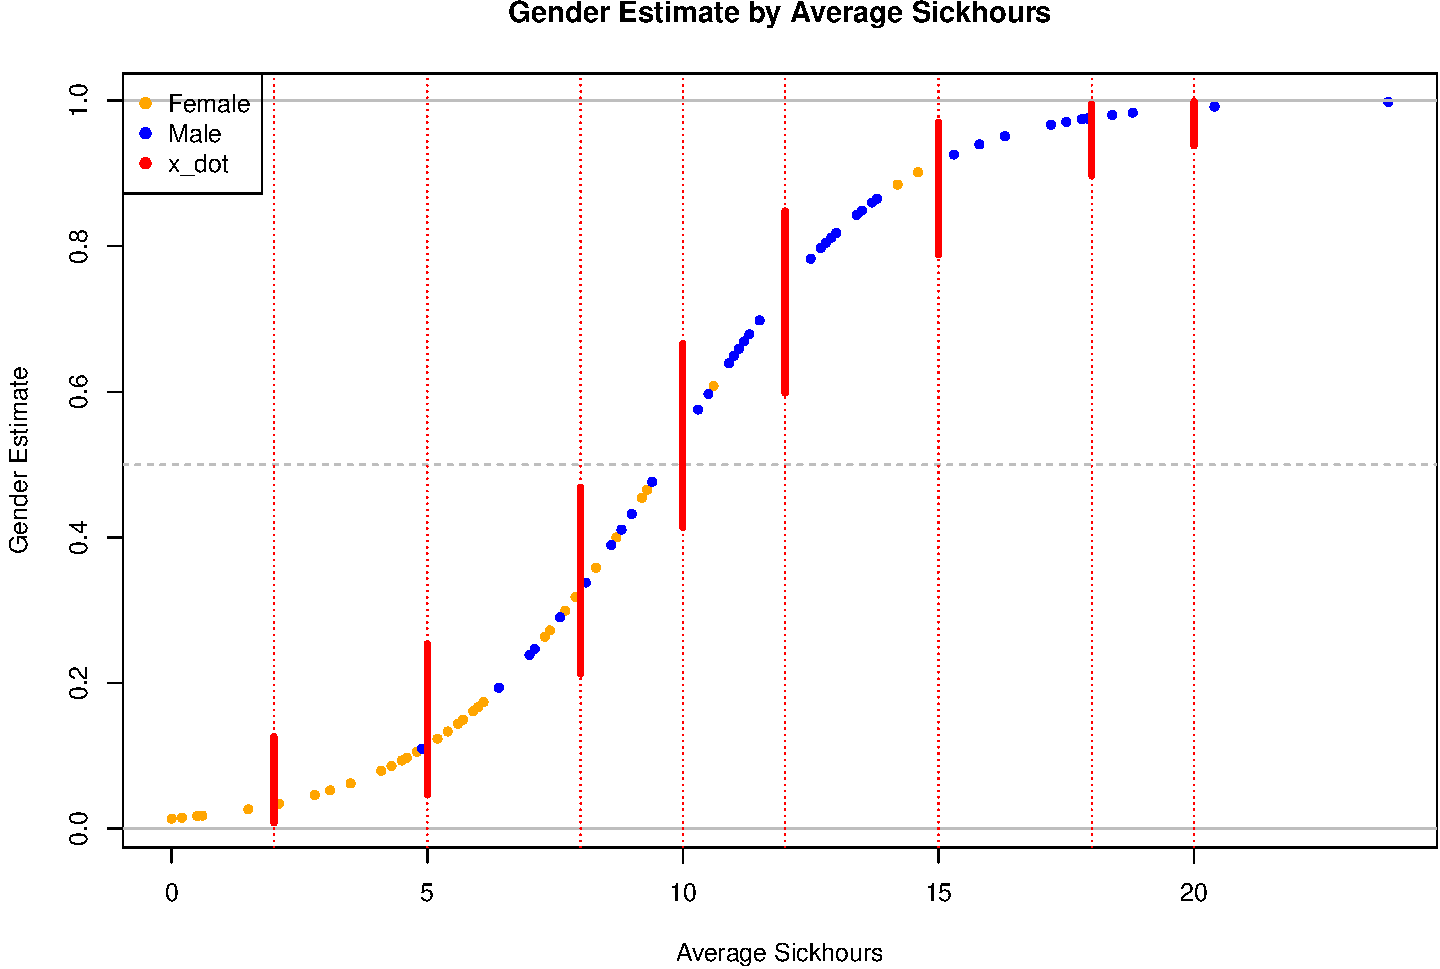
\includegraphics{Schmitt_Marvin_binary_response_files/figure-beamer/unnamed-chunk-24-1.pdf}
\normalsize

\end{frame}

\begin{frame}[fragile]

\begin{itemize}
\tightlist
\item
  \textbf{Alternative:} Equip the odds ratio of \(\beta\) with a
  confidence interval:

  \begin{itemize}
  \tightlist
  \item
    95\% CI:
    \([\exp(\hat{\beta}-1.96\hat{\sigma_{\beta}}), \exp(\hat{\beta}+1.96\hat{\sigma_{\beta}})]\)
  \item
    Invariant to the value of \(\dot{x}\)
  \item
    Typically reported in clinical research papers.
  \end{itemize}
\end{itemize}

\tiny

\begin{Shaded}
\begin{Highlighting}[]
\NormalTok{m =}\StringTok{ }\KeywordTok{glm}\NormalTok{(gender}\OperatorTok{~}\NormalTok{avg_sickhours, }\DataTypeTok{data=}\NormalTok{df, }\DataTypeTok{family=}\KeywordTok{binomial}\NormalTok{(}\StringTok{'logit'}\NormalTok{))}
\NormalTok{pred =}\StringTok{ }\KeywordTok{predict}\NormalTok{(m,}\DataTypeTok{newdata=}\KeywordTok{data.frame}\NormalTok{(}\DataTypeTok{avg_sickhours=}\DecValTok{10}\NormalTok{),}\DataTypeTok{se=}\NormalTok{T)}
\KeywordTok{c}\NormalTok{(}\KeywordTok{exp}\NormalTok{(pred}\OperatorTok{$}\NormalTok{fit}\FloatTok{-1.96}\OperatorTok{*}\NormalTok{pred}\OperatorTok{$}\NormalTok{se.fit), }\KeywordTok{exp}\NormalTok{(pred}\OperatorTok{$}\NormalTok{fit}\FloatTok{+1.96}\OperatorTok{*}\NormalTok{pred}\OperatorTok{$}\NormalTok{se.fit))}
\end{Highlighting}
\end{Shaded}

\begin{verbatim}
##         1         1 
## 0.7068071 1.9941010
\end{verbatim}

\normalsize

\end{frame}

\begin{frame}[fragile]{Other link functions}
\protect\hypertarget{other-link-functions}{}

\tiny

\begin{Shaded}
\begin{Highlighting}[]
\NormalTok{mlogit    =}\StringTok{ }\KeywordTok{glm}\NormalTok{(gender }\OperatorTok{~}\StringTok{ }\NormalTok{avg_sickhours, }\DataTypeTok{data =}\NormalTok{ df, }\DataTypeTok{family =} \KeywordTok{binomial}\NormalTok{(}\DataTypeTok{link=}\StringTok{'logit'}\NormalTok{))}
\NormalTok{mprobit   =}\StringTok{ }\KeywordTok{glm}\NormalTok{(gender }\OperatorTok{~}\StringTok{ }\NormalTok{avg_sickhours, }\DataTypeTok{data =}\NormalTok{ df, }\DataTypeTok{family =} \KeywordTok{binomial}\NormalTok{(}\DataTypeTok{link=}\StringTok{'probit'}\NormalTok{))}
\NormalTok{mcloglog  =}\StringTok{ }\KeywordTok{glm}\NormalTok{(gender }\OperatorTok{~}\StringTok{ }\NormalTok{avg_sickhours, }\DataTypeTok{data =}\NormalTok{ df, }\DataTypeTok{family =} \KeywordTok{binomial}\NormalTok{(}\DataTypeTok{link=}\StringTok{'cloglog'}\NormalTok{))}
\NormalTok{mcauchit  =}\StringTok{ }\KeywordTok{glm}\NormalTok{(gender }\OperatorTok{~}\StringTok{ }\NormalTok{avg_sickhours, }\DataTypeTok{data =}\NormalTok{ df, }\DataTypeTok{family =} \KeywordTok{binomial}\NormalTok{(}\DataTypeTok{link=}\StringTok{'cauchit'}\NormalTok{))}
\end{Highlighting}
\end{Shaded}

\normalsize

\tiny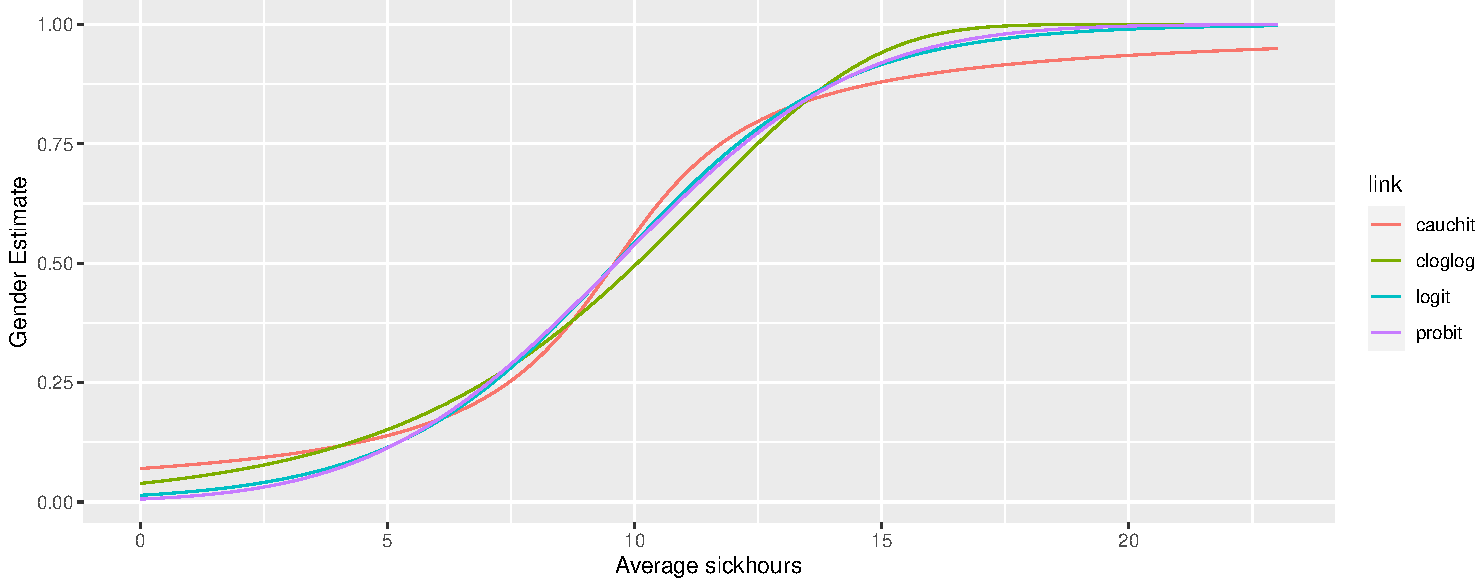
\includegraphics{Schmitt_Marvin_binary_response_files/figure-beamer/unnamed-chunk-27-1.pdf}
\normalsize

\end{frame}

\begin{frame}

\textbf{How to choose an appropriate link function?}

\begin{itemize}
\tightlist
\item
  Usually, most observed data lies in the center of the distribution.
\item
  Different link functions are typically similar in the center but
  differ in the \textbf{tails}.
\item
  \textbf{Approach:} Select the link function based on \emph{theoretical
  assumptions}, \emph{experience}, and \emph{domain expertise}.
\end{itemize}

\end{frame}

\begin{frame}{Questions?}
\protect\hypertarget{questions}{}

\end{frame}

\end{document}
